\begin{frame}{Permutation}
    \begin{block}{Definition}<1->
    A \emph{permutation} $\pi$ is a bijection between a set and itself.
    \end{block}
    \begin{block}{Example}<2->
        The permutations of size $3$ are
        \[
            123, 132, 213, 231, 312, 321.
        \]
    \end{block}
    \onslide<3->{%
    \begin{figure}
    \centering
    
    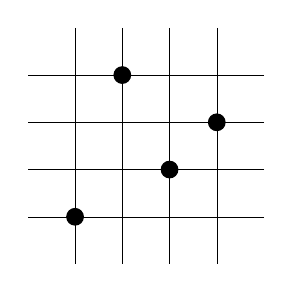
\begin{tikzpicture}[,scale=0.6, every node/.style={scale=0.6}]
            \foreach \x in {1,...,4} {
                    \draw[ultra thin] (\x,5)--(\x,0);
                    \draw[ultra thin] (5,\x)--(0,\x);
            }
            \draw[fill=black] (1,1) circle (5pt);
            \draw[fill=black] (2,4) circle (5pt);
            \draw[fill=black] (3,2) circle (5pt);
            \draw[fill=black] (4,3) circle (5pt);
    \end{tikzpicture}
    \caption{The graphical representation of $\pi=1423$.}
    \end{figure}
    }
\end{frame}